\section{Ricerca della costante elastica della molla: metodo statico}

\subsection{Apparato sperimentale}
L'apparato sperimentale utilizzato è costituito da:
	\begin{itemize}
		\item{una base ad A che sostiene un'asta verticale dotata di gancio di sospensione
            per le molle e asta millimetrata scorrevole. L'asta millimetrata ha sul lato sinistro
            una scala con una risoluzione di mezzo millimetro, mentre sul lato destro una scala con
            una risoluzione di un millimetro.}
		\item{quattro molle elicoidali con costanti elastiche differenti tra di loro: nello specifico
            una particolarmente ``morbida'', una ``dura'' e due con caratteristiche intermedie.}
		\item{un piattello portapesi di massa $m_{piattello} = 25.2\,\,g \pm\, 0.1\,\,g$, quattro pesi
            cilindrici neri rispettivamente di massa nominale 5, 10, 25 e 50 grammi e quattro pesi argentei
            analoghi a quelli neri, con le stesse masse nominali.}
        \item{una bilancia elettronica con una risoluzione di 0.1 grammi.}
	\end{itemize}

\subsection{Procedura di aquisizione dei dati}

Poiché una forza F di trazione o compressione applicata ad una molla elicoidale provoca una deformazione del corpo ed una conseguente risposta elastica, abbiamo deciso di sfruttare come forza agente la forza peso $F_{p}$ delle masse cilindriche a nostra disposizione. Per fare questo ricordiamo che la relazione tra una massa inerziale e la forza peso è la seguente:

\begin{equation}
	F_{p} = mg
    \label{eq:fp}
\end{equation}
%
dove g rappresenta l'accelerazione di gravità che assumiamo avere un valore $g = 9.806\,\,m\,s^{-2}$ e di cui trascuriamo l'incertezza.

La molla risponde all'allungamento dovuto alla forza $F_p$ con una forza $F_{el}$ uguale e contraria
data dalla (\ref{eq:hooke}),
per cui si ottiene $F_p = kx$. Applicando alla molla diverse masse e quindi diverse forze peso è possibile risalire al valore di $k$.

Innanzitutto abbiamo deciso di applicare alla molla 13 masse da 5 g a 125 g circa, suddividendo l'intervallo in modo equispaziato.
Sono quindi state selezionate tredici combinazioni di masse cilindriche aventi le masse scelte.
Per evitare di dover propagare gli errori sulla massa delle combinazioni, invece di misurare la massa di ogni singolo cilindro,
si è misurata la massa complessiva di ogni combinazione.
Abbiamo annotato quali cilindri facevano parte di ogni combinazione, in modo da poter ricomporre gli accoppiamenti in un secondo momento. Le masse totali delle combinazioni sono riportate nella tabella \ref{tab:masse}.

\begin{table}[tb]
    \centering
    \small
    \begin{tabular}{l | c c c c c c c c c c c c c}
        \multicolumn{14}{c}{\textbf{Masse delle combinazioni di cilindri [g]}} \\[1mm]
        \toprule
        Nominali & 5 & 15 & 25 & 35 & 45 & 55 & 65 & 75 & 85 & 95 & 105 & 115 & 125 \\
        Pesate & 5.0 & 15.1 & 24.9 & 35.0 & 45.2 & 55.1 & 65.2 & 75.0 & 85.1 & 95.2 & 105.0 & 115.2 & 125.3 \\
        \bottomrule
    \end{tabular}
    \caption{Masse usate per misurare l'allungamento della molla. Le masse erano composte da combinazioni
    di cilindri da 5, 10, 25 e 50 grammi di massa nominale. Nella seconda riga sono riportati le masse
    rilevate con la bilancia, che in alcuni casi differiscono da quelli nominali, riportati nella prima riga.
    I valori riportati sono i valori di lettura dello strumento (che ha risoluzione 0.1 grammi). L'incertezza tipo sulle misure
    è 0.03 g.}
    \label{tab:masse}
\end{table}

Per misurare la massa dei dischetti a nostra disposizione abbiamo utilizzato una bilancia elettronica con una risoluzione di 0.1 grammi. Abbiamo osservato che lo strumento era abbastanza sensibile da rilevare variazioni nella pressione dell'aria circostante. Lo abbiamo appurato soffiandoci sopra e notando che il valore rilevato dalla bilancia aumentava in modo considerevole. Per questo motivo per trovare le varie masse dei nostri pesi ci siamo assicurati di stare lontani dalla bilancia e di evitare di scuotere il tavolo di lavoro.

Completata la classificazione dei pesi, abbiamo scelto la molla di cui calcolare la
costante elastica. Abbiamo notato che una di esse era molto ``morbida'' per i carichi che saremmo
andati ad applicare e si deformava visibilmente anche con carichi piccoli, rendendo impossibili
le misure di deformazione dei carichi più grandi per questioni di spazio.
La abbiamo quindi scartata, anche perché sarebbe stata suscettibile di deformazione
plastica che avrebbe compromesso la buona riuscita dell'esperimento.
Un'altra molla è stata scartata in quanto troppo rigida: le sue deformazioni infatti non sarebbero state apprezzabili con carichi leggeri. Per questi motivi la scelta è ricaduta sulla molla tra 
le due restanti che permetteva una migliore lettura della deformazione in relazione ai pesi.

Per effettuare le misure, abbiamo agganciato il sistema molla-piattello al gancio di sospensione dell'asta verticale, lungo l'asta millimetrata. Atteso che l'oscillazione della molla si smorzasse, il bordo inferiore del piattello agganciato alla molla è stato allineato con la tacca dei 50 cm dell'asta graduata. In questo modo la posizione di equilibrio della molla senza carico risulta essere:

\begin{equation*}
	z_0\,\pm\,\delta z_0 = 50.00\,\pm\,0.03\,cm
\end{equation*}
%
per la quale abbiamo deciso di usare come incertezza l'errore tipo di risoluzione e la risoluzione è pari ad 1 mm.
Infine abbiamo misurato l'allungamento della molla al variare delle combinazioni di cilindretti scelte. Ad ogni variazione del carico si è aspettato che le oscillazioni del sistema si smorzassero prima di effettuare la lettura dell'asta graduata. La lettura è stata effettuata sul lato dell'asta con risoluzione di un millimetro, poiché non siamo riusciti ad apprezzare i mezzi millimetri a causa delle oscillazioni della molla, che per quanto piccole erano sempre presenti. Così facendo abbiamo ottenuto una serie di misure delle diverse posizioni di equilibrio della molla

\begin{equation*}
	z_i\,\pm\,\delta z
\end{equation*}
%
dove $\delta z \,=\, 0.3$ mm indica l'errore tipo di risoluzione, uguale per tutte le misure.

\subsection{Elaborazione dei dati}

\subsubsection{Considerazioni inziali e incertezze}
\label{incertezze}

Come detto precedentemente, la massa dei nostri tredici pesi è data da composizioni dei cilindretti a nostra disposizione e ognuno di essi è affetto da un errore sulla sua massa, dovuto alla risoluzione della bilancia. Per evitare di dover propagare le incertezze delle singole masse alle loro somme, abbiamo misurato la massa di ogni composizione cosicché risultasse affetta soltanto dall'errore di risoluzione dello strumento. Quindi le masse sono tutte affette dalla stessa incertezza tipo di risoluzione, che vale

\begin{equation*}
	\delta m \,=\, \frac{1}{\sqrt{12}}\Delta m \,\simeq\, 0.03 \,g 
\end{equation*}
%
dove $\Delta m = 0.1$ g indica la risoluzione dello strumento.

L'allungamento della molla è proporzionale alla forza ad essa applicata, cioè la forza peso, che è stata calcolata con la relazione (\ref{eq:fp})
dove è stato assunto il valore $g = 9.806 \,\, m/s^2$ e si è trascurata la sua incertezza. I pesi ottenuti sono riportati nella
prima colonna della tabella \ref{tab:dati}.

Dal momento che, per calcolare la costante elastica della molla, siamo costretti a passare per la relazione $F_p = k\,x$, in cui entra la forza peso e non la massa, dobbiamo propagare l'incertezza dalla misura della massa alla forza peso applicata alla molla. Si ottiene quindi la relazione:

\begin{equation*}
	\delta F_{p}\, =\, g\,\delta m \,=\, 0.0003 \,\, N 
\end{equation*}
%
L'allungamento della molla all'applicazione della massa $i$-esima è dato dalla differenza tra la posizione finale $z_i$ e quella di equilibrio $z_0$:

\begin{equation*}
	x_i = |z_i\,-\,z_0|
\end{equation*}
%
Gli allungamenti calcolati sono riportati in tabella \ref{tab:dati}. L’incertezza sugli allungamenti $\delta x$, che è uguale per tutte le misure, si ricava applicando la regola per la propagazione delle incertezze sulla differenza di misure indipendenti:

\begin{equation*}
	\delta x = \sqrt{\delta z^2\, + \,\delta z_0^2} \,=\, 0.0004 \,\, m
\end{equation*}
%
Da notare che la posizione iniziale della molla è stata calcolata con il piattello portapesi già agganciato ad essa pertanto l'allungamento rilevato si riferisce soltanto alla massa applicata.

\begin{table}
    \centering
    \begin{tabular}{c c c c c c c}
        \multicolumn{7}{c}{\textbf{Pesi e allungamenti}} \\[1mm]
        \toprule
        Massa [g] & Pos. eq. [cm] & Peso [N] & Allungamenti [m] & $k$ [$\frac{N}{m}$] & $\delta k$ [$\frac{N}{m}$] & $\delta k_x$ [$\frac{N}{m}$]\\
        \midrule
        5.0 & 49.5 & 0.049 & 0.005 & 9.8 & 0.8 & 0.8 \\
		15.1 & 48.4 & 0.148 & 0.016 & 9.3 & 0.2 & 0.2 \\
		24.9 & 47.4 & 0.244 & 0.026 & 9.4 & 0.1 & 0.1 \\
		35.0 & 46.4 & 0.343 & 0.036 & 9.5 & 0.1 & 0.1 \\
		45.2 & 45.3 & 0.443 & 0.047 & 9.43 & 0.08 & 0.08 \\
		55.1 & 44.3 & 0.540 & 0.057 & 9.48 & 0.07 & 0.07 \\
		65.2 & 43.3 & 0.639 & 0.067 & 9.54 & 0.06 & 0.06 \\
		75.0 & 42.4 & 0.735 & 0.076 & 9.68 & 0.05 & 0.05 \\
		85.1 & 41.4 & 0.834 & 0.086 & 9.70 & 0.05 & 0.05 \\
		95.2 & 40.4 & 0.934 & 0.096 & 9.72 & 0.04 & 0.04 \\
		105.0 & 39.3 & 1.029 & 0.107 & 9.62 & 0.04 & 0.04 \\
		115.2 & 38.3 & 1.130 & 0.117 & 9.66 & 0.03 & 0.03 \\
		125.3 & 37.3 & 1.229 & 0.127 & 9.67 & 0.03 & 0.03 \\
        \bottomrule
    \end{tabular}
    \caption{La tabella riassume i dati raccolti ed i calcoli eseguiti. La prima colonna elenca le masse delle combinazioni, riportate anche in tabella
        \ref{tab:masse}, mentre la seconda colonna riporta le posizioni di equilibrio $z_i$ misurate per le rispettive masse.
        La terza colonna riporta i pesi in Newton 
        delle masse appese alle molle (calcolati con il valore $g = 9.806 \,\, m/s^2$), la quarta i relativi allungamenti $x_i$.
        Le incertezze sui valori delle prime tre colonne sono calcolate nel paragrafo \ref{incertezze}.
        La quinta colonna riporta il valore di k stimato facendo il rapporto $P_i/x_i$ della relativa riga. Le ultime due colonne
        riportano le incertezze sul k ricavate con la propagazione degli errori. Nell'ultima colonna è stato trascurato il contributo
        dell'incertezza sul peso, che, come si può vedere facilmente, non è significativa. \emph{Nota:}
        I dati delle prime quattro colonne sono approssimati come da risoluzione degli strumenti usati, anche se i loro errori standard
        sono di un ordine di grandezza inferiore. Non avrebbe molto senso mettere una cifra in più in quanto va oltre la risoluzione degli
        strumenti e non porta informazione.}
    \label{tab:dati}
\end{table}

\begin{table}
    \centering
	\begin{tabular}{ c c  c  c  c  c }
        \multicolumn{6}{c}{\textbf{Carico e scarico della molla}} \\[1mm]
        \toprule
        \multirow{2}*{Massa [g]} & \multicolumn{5}{c}{Allungamenti [cm]} \\
        \cmidrule{2-6}
        & Prima misura & Carico 1	& Scarico 1	& Carico 2	& Scarico 2 \\
        \midrule
        15.1		& 1.6 & 1.5		& 1.5			& 1.5		& 1.5	\\
        35.0		& 3.6 & 3.5		& 3.5			& 3.5		& 3.5	\\
        55.1		& 5.7 & 5.6		& 5.6			& 5.5		& 5.6	\\
        75.0		& 7.6 & 7.5		& 7.5			& 7.5		& 7.6	\\	
        95.2		& 9.6 & 9.6		& 9.6			& 9.6		& 9.6	\\
        115.2		& 11.7 & 11.6		& 11.6			& 11.6		& 11.6	\\
        \bottomrule
	\end{tabular}
    \caption{La tabella mostra gli allungamenti della molla registrati durante le misurazioni effettuate per l'esperimento
        (prima misura, riportate anche in tabella \ref{tab:dati}), e durante i due cicli di carico-scarico.
        Tutte le misure sono affette dall'incertezza standard di
        risoluzione sulla lunghezza pari a 0.3 mm.}
    \label{tab:carico_scarico}
\end{table}

\subsubsection{Carico e scarico della molla}

In tutto il resto dell'esperimento abbiamo assunto che la molla non si deformasse (ovvero che fosse in regime elastico)
e che non cambiassero le posizioni di equilibrio relative alle diverse masse. Affinchè queste ipotesi risultino fondate,
abbiamo dovuto verificare che le posizioni di equilibrio delle masse non varino a seconda che vengano misurate durante la fase di carico
o scarico della molla. La tabella \ref{tab:carico_scarico} mostra la posizione di equilibrio per alcune masse applicate ed è stata realizzata con una procedura di carico e scarico della molla. Ovvero: per le masse scelte si è deciso di caricare la molla e rilevare le varie posizioni di equilibrio, stessa cosa si è fatta nello scariare la molla. Questa procedura è stata ripetuta due volte.
Come si può intuire da una prima analisi qualitativa della tabella, risulta evidente che le misure sono compatibili tra di loro e questo ci porta a dire che la molla non è stata affetta da una deformazione dovuta ad un carico eccessivo. Si può inoltre osservare che i risultati non dipendono dalla procedura con cui è stato misurato l'allungamento (carico o scarico).
Affermiamo questo perchè prendendo per esempio la massa da ``55 g'' possiamo oservare che le varie misure sono le seguenti:
\begin{itemize}
	\item{primo allungamento $x_{all_1}$ = $5.7 \pm 0.03 \,\,cm$}
	\item{secondo allungamento $x_{all_2}$ = $5.6 \pm 0.03 \,\,cm$}
	\item{terzo allungamento $x_{all_3}$ = $5.6 \pm 0.03 \,\,cm$}
	\item{quarto allungamento $x_{all_4}$ = $5.5 \pm 0.03 \,\,cm$}
	\item{quinto allungamento $x_{all_5}$ = $5.6 \pm 0.03 \,\,cm$}
\end{itemize}
quindi facendo una media gli ultimi quattro allungamenti, che sono stati ricavati dalla proceura di carico e scarico ricaviamo che

RIVEDERE QUESTO PEZZO CON PASA E BUZZ !!!!!!!!

\begin{equation*}
	m^*[x_{all_i}] = \frac{1}{4} \sum_{i=2}^{5} (x_{all_i}) = 5.57\, cm
\end{equation*}
%
e l'incertezza su questo valore è la seguente:

\begin{equation*}
	\sigma^*[m^*[x_{all_i}]] = \sqrt{\frac{1}{4} \sum_{i=2}^{5} (x_{all_i} - m^*[x_{all_i}])^2} = 0.04 \,cm
\end{equation*}
%
Con questi valori possiamo pertanto valutare se la media delle misure ottenute dalla procedura di carico e scarico è compatibile con la misura ottenuta durante il primo ciclo di misurazione. Posto a priori un fattore di copertura k = 3 andiamo a verificare che il resto tra la differenza fra $m^*[x_{all_i}]$ e $x_{all_1}$ risulti essere minore dell'errore relativo al resto moltiplicato per il fattore di copertura.
Otteniamo quindi:

\begin{equation*}
	R = x_{all_1} - m^*[x_{all_i}] = 0.13 \,\,cm
\end{equation*}

\begin{equation*}
	k\, \sigma_{R} = k\,\, \sqrt{(\sigma[x_{all_1}])^2 + (\sigma[m^*[x_{all_i}]])^2} = 0.15 \,\,cm
\end{equation*}
%
Da questo quindi possiamo dire che $m^*[x_{all_i}]$ e $x_{all_1}$ risultano essere compatibili, e compatibili sono anche le misure che abbiamo ottenuto per fare la media dei cicli di scarico e carico, sempre utilizzando come fattore di copertura il k scelto in precedenza.
Poiché tale procedura si può estendere anche a tutte le altre misure relative alle masse ottenendo le stesse conclusioni, possiamo dedurre che le misure sono tra di loro compatibili e non ci sono state deformazioni della molla.
Un'importante osservazione che si può fare analizzando la tabella \ref{tab:carico_scarico} è che per lo stesso carico applicato alla molla le misure dell'allungamento differiscono tra di loro per 0.1 cm. Abbiamo ipotizzato che questa differenza possa essere dovuta principalmente a due elementi:

\begin{enumerate}
	\item{dal momento che prima di effetuare i cicli di carico e scarico la molla era stata tolta dal supporto assieme al piattello portapesi, è probabile che nel riposizionare l'apparato l'allineamento del piattello portapesi, nella sua posizione di equilibrio, con la tacca dei 50 cm non sia stato perfetto ma sia risultato errato di 0.1 cm;}
	\item{un'altra possibilità è data da eventuali errori di parallasse, che non sono da escludere, in quanto riuscire a guardare correttamente tra il bordo inferiore e l'asta millimtrata non è un'operazione così elementare come può sembrare;}
\end{enumerate}

\subsubsection{Calcolo della costante elastica elastica a partire dalla tabella}

La procedura per il calcolo della costante elastica da noi seguita è il seguente:
per ogni massa usata si è stimato il valore della costante $k_i$ facendo il rapporto $k_{i} = \frac{F_{p_{i}}}{x_{i}}$,
e i valori ottenuti sono stati utilizzati per ricavare un unico valore di $k$ mediante due procedure: la media pesata e il metodo statistico.
L'incertezza $\delta k_{i}$ su ogni valore $k_i$ è stata calcolata mediante la regola per la propagazione delle incertezze sui rapporti di misure indipendenti:

\begin{equation*}
	\left(\frac{\delta {k_{i}}}{k_{i}}\right)^2 = \left(\frac{\delta F_{p_{i}}}{F_{p_{i}}}\right)^2 + \left(\frac{\delta_{x_{i}}}{x_{i}}\right)^2 
\end{equation*}
%
da cui segue

\begin{equation}
	\delta k_{i} \,=\, k_i\,\, \sqrt{\left(\frac{\delta F_{p_{i}}}{F_{p_{i}}}\right)^2 + \left(\frac{\delta_{x_{i}}}{x_{i}}\right)^2} 
    \label{eq:deltaki}
\end{equation}
%
I valori $k_i$ calcolati e le relative incertezze sono riportati in tabella \ref{tab:dati}. Da notare che le incertezza
non risultano essere tutte uguali, poichè nella formula (\ref{eq:deltaki}) sono presenti le incertezze relative, che
variano per ogni massa. Notiamo inoltre che le incertezze relative sul peso sono trascurabili, infatti eliminado il termine
$\left(\frac{\delta F_{p_{i}}}{F_{p_{i}}}\right)^2$ dalla (\ref{eq:deltaki}) i valori delle incertezze $\delta k_i$ non variano.
I valori delle incertezze ottenute trascurando l'errore sul peso sono riportati nell'ultima colonna della tabella \ref{tab:dati}.

Vediamo ora come abbiamo ottenuto il valore $k$ tramite i due metodi accennati sopra.

\paragraph{Primo metodo: Media pesata\\}

Il primo metodo che prendiamo in considerazione è quello di calcolare la media pesata dei valori $k_{i}$ e per farlo ci serviremo delle seguenti formule:

\begin{equation*}
    k_{0,w} = \frac{\sum (k_i w_i)}{\sum (w_i)} , \quad \delta k_{w} = \frac{1}{\sqrt{\sum (w_i)}} , \qquad \text{dove} \quad w_i = \frac{1}{(\delta k_i)^2}
\end{equation*}
%
in particolare $k_0$ appresenta il risultato della media pesata delle varie costanti elastiche $k_i$ ottenute, $\delta k_0$ simboleggia l'errore relativo a $k_0$ e $w_i$ è il peso relativo alla misura $k_i$, ovvero quanto quella misura contribuisce nella media complessiva. E' importente sottolineare che la procedura non è in grdo di tenere conto di eventuali altre sorgenti di incertezza come ad esempio un errore sistematico.

Quindi con i dati a nostra disposizione abbiamo otteuto il seguente risultato:

\begin{equation}
    k_{0,w} \,\, \pm \,\, \delta k_{w} =  9.64 \,\, \pm \,\, 0.01 \,\,N/m
    \label{eq:w}
\end{equation}

\paragraph{Secondo metodo: Distribuzione dei valori di $k_i$\\}
Il secondo metodo che addottiamo per il calcolo della costante elastica della molla elicoidale è quello di considerare la distribuzione dei valori $k_i$, ovvero se ne deve calcolare la media campionaria $m^*_k$ e stimarne lo scarto quadratico medio della distribuzione delle medie. In questo modo otteniamo:

\begin{equation*}
    k_{0,s} \,\,=\,\, m^*_k \,\,=\,\, \frac{1}{N}\,\,\sum_{i=1}^{N} (k_i) \,\,=\,\, 9.58  \,N/m
\end{equation*}
%
\begin{equation*}
    \delta k_{s}  \,=\, \frac{1}{\sqrt{N}} \sigma_{k} \,=\, \frac{1}{\sqrt{N}}\sqrt{\frac{1}{N - 1}\,\,\sum_{i=1}^{N} (k_i - m^*_k)^2}\,=\, 0.04 \,\,N/m
\end{equation*}
%
ottenendo la misura:

\begin{equation}
    k_{0,s} \, \pm \, \delta k_{s} \,=\, 9.58 \,\, \pm \,\, 0.04 \,\, N/m
    \label{eq:s}
\end{equation}
%
Mettendo a confronto queste due procedure e aiutandoci con i dati riportati in tabella possiamo osservare che la media pesata sembrerebbe essere la procedura che meglio approssima il risultato dell'esperimento. Affermiamo questo perchè dalla tabella \ref{tab:dati} si può osservare che le prime stime della costante elastica risultano avere un incertezza molto superiore (fino a quasi 30 volte) alle altre misure effettuate. Una così grande differenza di precisione è dovuta al fatto che nella formula (\ref{eq:deltaki}) sono presenti le incertezze relative su peso ed allungamento. Poichè l'errore di risoluzione è uguale per tutte le misure, l'incertezza relativa è molto maggiore per le misure più piccole.  È quindi doveroso che nel calcolo di $k_0$ si tenga in considerazione della differente accuratezza delle misure dando più importanza a quelle con un incertezza inferiore rispetto alle altre.

\paragraph{Compatibilità delle costanti elastiche trovate\\}

Altra importante osservazione da fare è che le due misure (\ref{eq:w}) e (\ref{eq:s}) della costante elastica ottenute con queste due procedure risultano essere comatibili in quanto, fissato un fattore di copertura k = 3, a priori, otteniamo:
\begin{itemize}
	\item{la differenza tra i due $k_0$ risulta essere: $R \,=\, 0.06 \,\, N/m$}
	\item{l'errore relativo alla differenza dei due $k_0$ e la seguente:
            
        $$k \, \sigma_R = \sqrt{\delta k_{0,w}^2 + \delta k_{s}^2} = 0.12 \,\, N/m$$}
\end{itemize}
pertanto dal momento che $ R \leq k \, \sigma_R$ i due risultati della costante elastica sono compatibili tra di loro.

\subsubsection{Calcolo della costante elastica K a partire dal grafico}

Ricordando le seguenti relazioni:

\begin{equation}
    x \,\,=\,\, bF_p \qquad \text{ovvero} \qquad F_p \,\,=\,\, kx \qquad \text{pertanto} \qquad b \,\,=\,\, \frac{1}{k}
\end{equation}
%
possiamo procedere al calcolo della costante elastica k a partire direttamente dal grafico. Poiché i punti sul grafico sono ricavati sperimentalmente e di conseguena sono affetti da incertezza, per trovare la retta che meglio approssima il loro andamento, possiamo seguire la seguente procedura.

\paragraph{Metodo della Regressione lineare\\}

Questa procedura si basa sul metodo dei minimi quadrati, ovvero serve a ricavare la stima migliore del coefficiente angolare b che è data dal valore che rende minima la discrepanza tra i dati sperientali $F_{p_i} \,\,e\,\, x_i$ e la retta $x \,=\, bF_p$.\\
Procediamo operativamente in questo modo:

\begin{itemize}
	\item{La funzione da minimizzare che misura la discrepanza è:
			\begin{equation}
                \sum_{i=1}^{N} \frac{(x_i - bF_{p_i})^2}{(\delta x\ped{tot})^2}	
                \label{eq:min_quad}
			\end{equation}
% questo commento serve!
            dove $\delta x\ped{tot}$ è l'incertezza totale sugli allungamenti, ottenuta sommando l'incertezza $\delta x$ e
            l'errore trasferito dal peso.
        }

    \item{Consideriamo come stima prelminare di $b$, da utilizzare per trasferire le incertezze sul peso alla lunghezza,
        il valore $b \,=\, 1/k_{0,s}$ che si ottiene utilizzando $k_{0,s}$, ottenuto dal metodo
        statistico. Pertanto abbiamo stimato $b = 1/9.58 \,\, m/N = 0.10 \,\, m/N$.
        Il trasferimento dell'incertezza si ottiene usando la formula:
        
        \begin{equation}
            \delta x\ped{tot} = \sqrt{\delta x^2 + \delta x\ped{tras}^2} \qquad \text{con} \quad \delta x\ped{tras} = b\,\delta F_p
            \label{eq:tras}
		\end{equation}

        Usando la stima di $b$ si ottiene $\delta x\ped{tras} \simeq 3 \cdot 10^{-5}$ m. Confrontando $\delta x\ped{tras}$
        con $\delta x = 4 \cdot 10^{-4}$ m, si ha che $\delta x\ped{tras}^2 \ll \delta x^2$ per cui nella (\ref{eq:tras})
        l'incertezza trasferita può essere trascurata, ottendendo $\delta x\ped{tot} = \delta x$.

        Notiamo inoltre che l'incertezza $\delta x\ped{tot}$ è la stessa per tutti i valori $x_i$.}

    \item{Quindi minimizzando il valore di (\ref{eq:min_quad}), otteniamo le segenti relazioni:
			\begin{equation*}
                b_0  \,=\,  \frac{\sum F_{p_i}  x_i}{\sum F_{p_i}^2} \,=\, 0.1037 \,\, \frac{m}{N} \quad \,\, e \quad\,\,
                \delta b  =  \frac{\delta x}{\sqrt{\sum F_{p_i}^2}} \,=\, 0.0002 \,\, \frac{m}{N}
			\end{equation*}

			e quindi sfruttando la regola della propagazione dell'incertezze sul quoziente abbiamo

			\begin{equation*}
				\frac{\delta k}{k} \,=\, \frac{\delta b}{b}
			\end{equation*}

			pertanto ricordando che $k \,=\, \frac{1}{b}$ possiamo ottenere i valori di
            $k_{0,r} = \frac{1}{b_0}$ e $\delta k_{r} = \frac{\delta b}{b} k$, infatti otteniamo:

			\begin{equation*}
                k_{0,r} \pm \delta k_r \,=\, 9.64 \pm 0.01 \,\,\frac{N}{m}
			\end{equation*}
			}
\end{itemize}

Possiamo notare che la costante elastica così ottenua è uguale a quella ottenuta con la media pesata. Questo è dovuto al fatto che le due procedure sono equivalenti.

\begin{SCfigure}
    \centering
    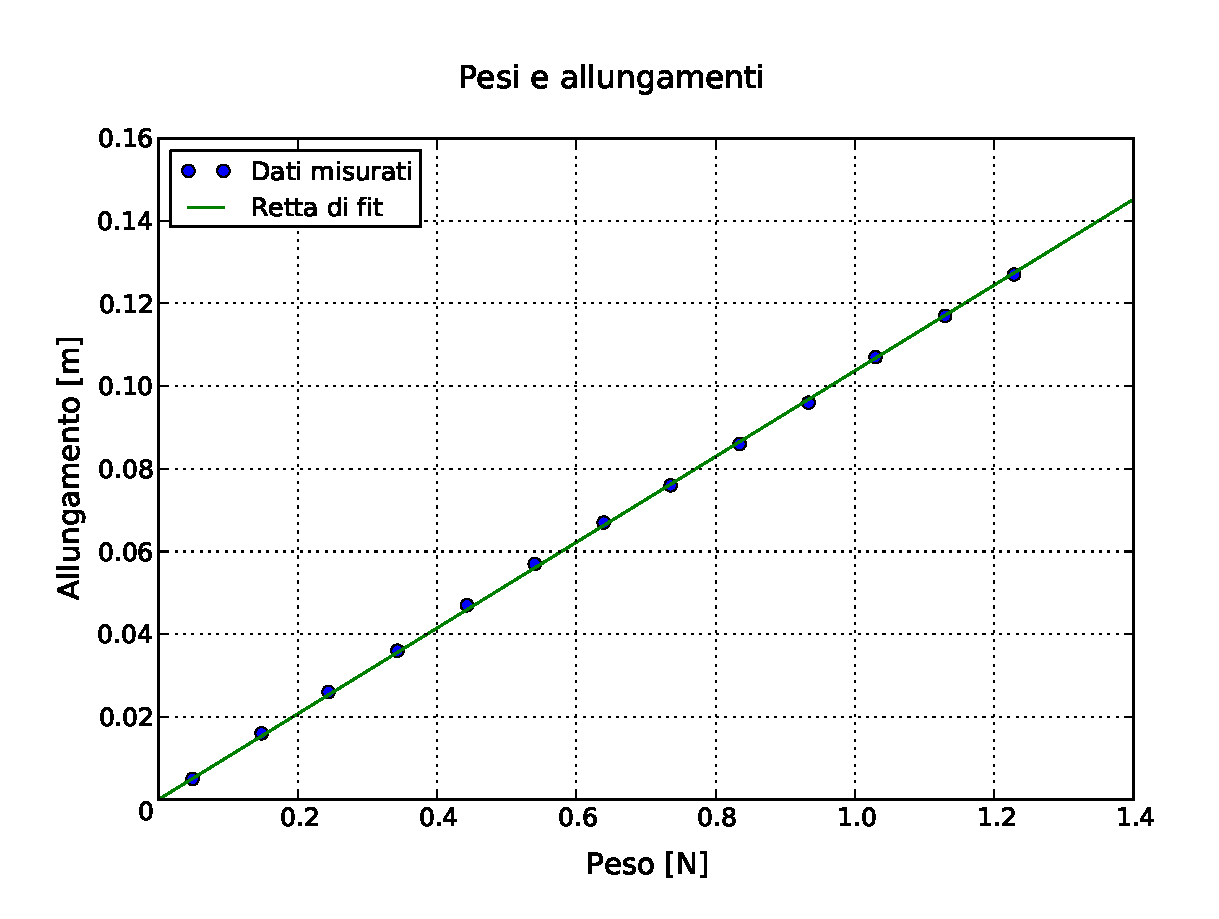
\includegraphics[width=120mm]{immagini/pesi_allungamenti.pdf}
    \caption{Plot massa versus allungamento della molla. Le barre di incertezza dei punti non sono mostrate,
        in quanto molto piccole (circa la dimensione dei pallini) e difficilmente leggibili. Si vede bene
        che l'allungamento è funzione lineare della massa. La retta verde è la retta di fit calcolata mediante la regressione lineare.}
    \label{fig:regressione}
\end{SCfigure}

\subsubsection{Test del chi quadro}

Fino a questo punto noi abbiamo valutato la compatibilità dei valori sperimentali con la legge di Hooke esaminando qualitativamente il grafico. Possiamo però valutare la compatibilità dei dati anche con un metodo quantitativo che si basa sul test del chi quadro. Questo test confronta, punto per punto, la discrepanza tra i valori sperimentali e la retta teorica
$(x_i - b-0 F_{p_i})$ e questo valore dovrebbe essere mediamente paragonabile con l'incertezza ($\delta x_i$) del singolo dato. Ricordiamo che la discrepanza viene calcolata sui valori che nel grafico saranno riportati sull'asse delle ordinate. Inoltre questa verificaparte dall'ipotesi, nel nostro caso verificata, che l'errore sui valori in ascissa sia trascurabile rispetto a quello sull'ordinata.
Procediamo quindi col test del chi quadro:

\begin{itemize}
\item{Calcoliamo il chi quadro (oss sta per osservato, ovvero calcolato dai dati sperimentali):

	\begin{equation*}
        \chi_{oss}^2 \,=\, \sum_{i=1}^{N} \frac{(x_i - b_0 F_{p_i})^2}{(\delta x)^2} = 29
	\end{equation*}
	%
	dove $b_0$ rappresenta il coefficiente angolare determinato, mediante la regressione lineare, nel paragrafo precedente.}
\item{Se il test va a buon fine ci si aspetterebbe che:

	\begin{equation*}
		\chi_{oss}^2 \, \simeq \, \chi_{teo}^2 \,=\, N - 1 \,=\, 12  
	\end{equation*}
	%
	ricordando che $\chi_{teo}^2 \equiv$ ``numero gradi di libertà del sistema'', che nel nostro caso sono $N - 1$ in
    quanto dobbiamo tener conto che un parametro della curva di fit, ovvero $b_0$, è stato ricavato a partire dai dati
    sperimentali. N rappresenta il numero di punti sperimentali.}
\item{L'incertezza sul chi quadro teorico vale:

    \begin{equation*}
        \delta\chi_{teo}^2 \,=\, \sqrt{2(N - 1)} = 5  
	\end{equation*}

    }
\end{itemize}
%
Si ha quindi:

\begin{equation*}
	\chi_{teo}^2 \pm \delta\chi_{teo}^2 \,\,=\,\, 12 \,\,\pm\,\, 5
\end{equation*}
%
andiamo a verificare che $\chi_{oss}^2$ sia compatibile con $\chi_{teo}^2$, premettendo che adotteremo, come
nel resto della relazione, un fattore di copertura k = 3:

\begin{equation*}
	|R| \,\, \leq \,\, k \, \delta\chi_{teo}^2 \qquad \text{dove} \quad |R| = |\chi_{teo}^2 - \chi_{oss}^2|
\end{equation*}
%

La differenza tra i due chi quadro risulta essere $|R| \,=\, 17$ che \emph{non} risulta essere minore di
$k \, \sigma \chi_{teo}^2 \,=\, 15$, pertanto i due chi quadro non sono compatibili.

Come prima cosa verificato che questo non fosse dovuto all'influenza di particolari punti sperimentali ad esempio il primo o l'ultimo.
A tal fine abbiamo controllato che la discrepanza tra il dato singolo e la predizione teorica non fosse molto maggiore di uno:

\begin{equation*}
	\frac{(x_i - b_0 F_{p_i})^2}{(\delta x)^2} \, \gg \, 1
\end{equation*}
%
Il grafico in figura \ref{fig:discrepanza_statico} mostra la discrepanza tra dati e retta di fit.
Si può vedere che non ci sono punti che contribuiscono in maniera esagerata rispetto ad altri al valore $\chi^2_{oss}$.

A questi punto le possibili soluzioni sono due: la prima è che i dati sperimentali non sono compatibili con la legge di Hooke, caso che ci sentiamo di escludere in quanto è stato provato ripetutamente che la legge in questione è valida. Perciò non rimane che ammettere di aver sottostimato le incertezze sugli allugamenti $x_i$.

\begin{SCfigure}
    \centering
    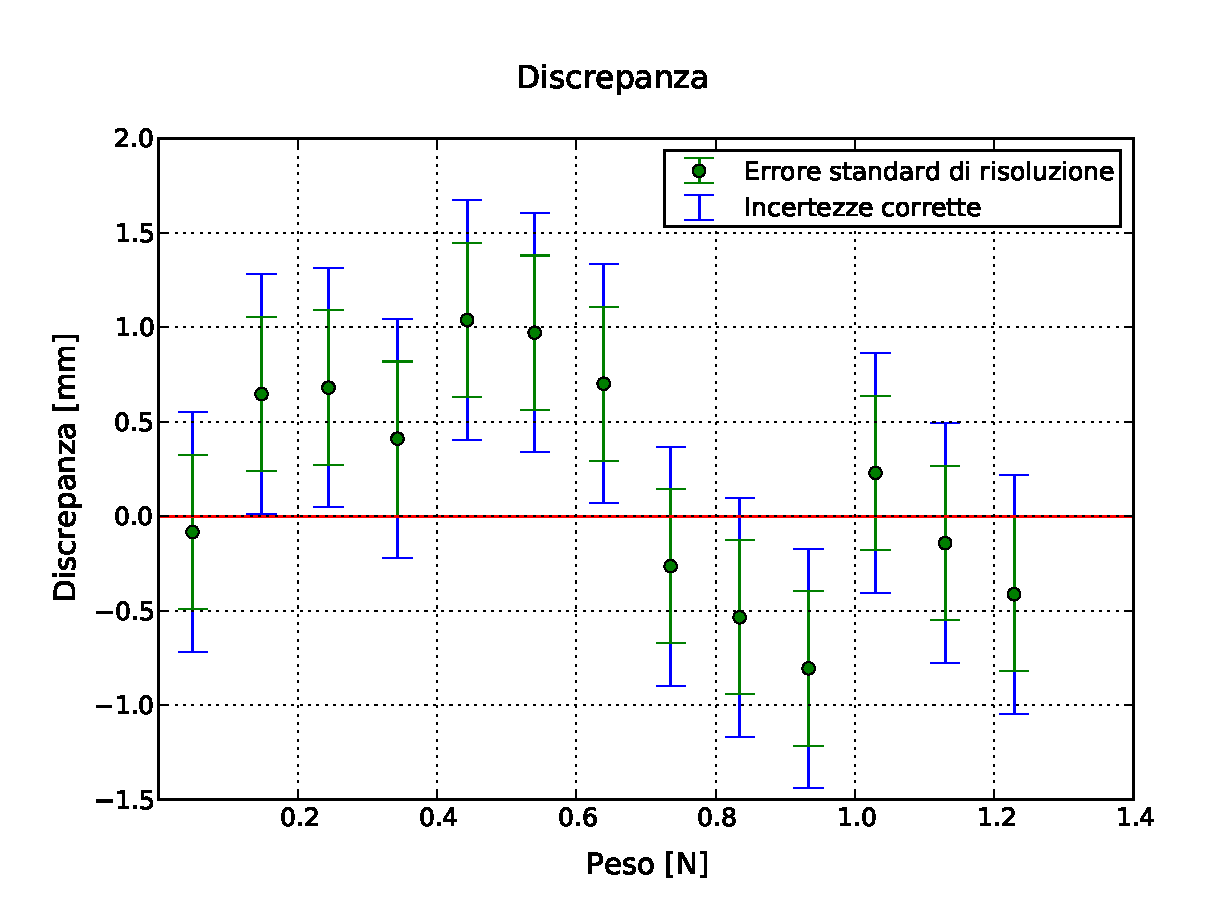
\includegraphics[width=120mm]{immagini/discrepanza_statico.pdf}
    \caption{La figura mostra la discrepanza tra i valori di allungamento misurati e la retta ottenuta col fit, in modo
        da rendere visibili le incertezze. Le barre di errore verdi mostrano l'errore calcolato a priori mentre
        le barre blu mostrano le incertezze corrette per far tornare il $\chi^2$. Le incertezze sono tutte uguali.
        Da notare il fatto che non si distingue alcun andamento residuo nei dati.}
    \label{fig:discrepanza_statico}
\end{SCfigure}

Si è deciso di aggiustare l'errore $\delta x$. Imponiamo che:

\begin{equation*}
    \chi_{oss}^2 \,=\, \sum_{i=1}^{N} \frac{(x_i - b_0 F_{p_i})^2}{(\delta x)^2} \,=\, \chi_{teo}^2 
\end{equation*}
%
da cui ricaviamo, grazie al fatto che le incertezze sono tutte di egual valore,

\begin{equation*}
    \delta x\ped{posteriori}^2 \,\,=\,\, \frac{\sum_{i=1}^{N} (x_i - b_0 F_{p_i})^2}{\chi_{teo}^2}
    %\chi_{oss}^2 \,=\, \frac{1}{(\delta x)^2} \sum_{1}^{N} (x_i - b_0 F_{p_i})^2  \,=\, \chi_{teo}^2
\end{equation*}
%
Poiché $\chi_{teo}^2 = 12.0$ si calcola facilmente che:

\begin{equation*}
    \delta x\ped{posteriori} \,=\, 0.0006 \,m \,\,=\, 0.6 \,\, mm
\end{equation*}
%
Abbiamo ottento che il $\chi_{oss}^2$ coincide con $\chi_{teo}^2$ dopo aver aumentato l'incertezza sugli allungamenti di un fattore
$s$.
Crediamo che questa variazione sia più che accettabile. Infatti come accennato all'inizio dell'analisi dei dati, la lettura
dell'allungamento non risultava così agevole a causa delle continue oscillazioni della molla, che è a tutti gli effetti
un oscillatore armonico. Inoltre, non abbiamo tenuto conto dell'errore di parallasse.\\
Dal momento che abbiamo variato l'errore sulla misura dell'allungamento otteniamo come nuovo valore della costante elastica della molla il seguente risultato:

\begin{equation*}
	k_0 \,\, \pm \,\, \delta k_0 \,\,=\,\, (9.64 \,\, \pm \,\, 0.02)\,\, N/m
\end{equation*}
%
dove ovviamente l'unico cambiamento riguarda l'incertezza sulla misura che risuta essere maggiore di quella calcolata in precedenza per ovvi motivi.\\

Quindi l'unica cosa che ci rimane da verificare è se questo nuovo valore di $K_0$ sia compatibile con i valore di $k_0$ trovato mediante la distribuzione dei $k_i$.
Pertanto abbiamo quanto segue:
\begin{itemize}
	\item{il resto (R) tra i due $k_0$ risulta essere: $R \,=\, 0.06 \,\, N/m$}
	\item{posto come fattore di copertura k = 3 abbiamo che $k \, \sigma_R$ risulta essere:
			\begin{equation*}
				k \, \sigma_R \,\,=\,\, 0.13 \, N/m
			\end{equation*}}
	\item{pertanto abbiamo che $|R| \,\, \leq \,\, k \, \sigma_R $ e quindi i due $k_0$ risultano essere compatibili}
\end{itemize}

